% В этом файле следует писать текст работы, разбивая его на
% разделы (section), подразделы (subsection) и, если нужно,
% главы (chapter).

% Предварительно следует указать необходимую информацию
% в файле SETUP.tex

\input{preamble.tex}

\begin{document}

\Intro

Здесь нужно написать введение.

% Если typeOfWork в SETUP.tex задан как 2 или 3, то начинать
% надо не с section (раздел), а с главы (chapter)
\chapter{Теоретические и практические подходы, применяемые для извлечения фактов из слабоструктурированных текстовых документов}
\section{Основные теоретические понятия}
\subsection{Понятие слабоструктурированного документа}
Под слабоструктурированными документами подразумеваются текстовые источники данных, которые характеризуются следующим набором признаков и свойств:
\begin{itemize}
  \item Документ содержит в том или ином виду внутреннюю разметку
  \item Разбиение содержимого документа на фрагменты средствами внутреннего форматирования
  \item Фрагменты документа представляют собой ифнормационные поля, либо же значения информационных полей
  \item По внутренней разметке документа нельзя однозначно определить, является ли фрагмент полем, либо же значением поля
\end{itemize}
В качестве примера слабоструктурированного документа можно взять договор. Договор как таковой характеризуется определенным набором информационных полей и их значений. Например, каждый договор должен содержать названия контрагентов, а также имена и должности физических лиц, подписывающих договор. Однако же в общем и целом два среднестатистических договора могут весьма значительно отличаться по структуре, по скольку правила оформления договоров оставляют довольно большое место для импровизации путем добавления/удаления тех или иных полей. В конечном счете нельзя однозначно сказать для заданного информационного поля, в какой части документа его искать и будет ли оно там вообще.

Также можно выделить неструктурированные документы и структурированные. Первые представляют собой текстовый документ произвольного формата. Вторые характеризуются строгим набором правил форматирования, который позволяет однозначно интерпретировать такие документы и извлекать из них информацию.

\chapter{Программная реализация}
\section{Общая структура проекта}
Разработонная программа явялется консольным приложением, которое принимает на вход файл с текстом документа вместе с набором правил, и возвращает последовательность пар (FiledName, FiledValue), где FiledName - название информационного поля (задается в файле с правилами), а FieldValue - его значение.

Схему работы программы можно видеть на рисунке \ref{fig:project-diagram}. Программа содержит три основных модуля: 
\begin{itemize}
  \item Модуль разбора и разметки входного текста
  \item Модуль разбора пользовательских правил
  \item Модуль построения GLR-парсера
\end{itemize}

Первый модуль обрабатывает входной текст. Текст очищается от лишних символов и разбивается на группы токенов так, что каждая группа соотвествует одному абзацу. Токены представляют собой последовательности букв и цифр, которые соотвествуют словам в тексте документа. Каждый токен анализируется и соотвествующим образом помечается. Например, сохраняется информация о части речи токена, и многих других морфологических харакетистиках. Для разметки используется библиотека pymorphy2. В конце формируется массив, содержащий упорядоченную последовательности групп токенов. Именно элементы этой последовательности затем принимает парсер.

Второй модуль обрабатывает пользовательские правила. Правила записываются в текстовый файл в строго опредленном формате. Файл быть размечен на две секции: секцию описания правил и секцию комманд. Первая секция предназанчена для описания пользовательских правил, вторая - для указания правил, которые нужно найти. Искомое правило должно быть либо определено вручную в секции правил, либо же являться встроенным. Полученный файл с правилом затем передается на обработку программе GNU Bison. Она обрабатывает файл, строит для него парсер по заранее заданной грамматике и разбирает, в процессе накапливая информацию об описанных правилах и командах.

Третий модуль непосредственно строит GLR-парсер, с помощью которого анализируется текст документа. На вход ему поступает информацию, накопленная в модуле разбора пользовательских правил. На основе полученной информации строится одна или несколько грамматик. Их количество зависит числа уникальных правил, которые помечены пользователем как цели для поиска. Затем для каждой из построенных построенных грамматик запускается процесс построения парсера, который состоит из нескольких этапов.
\begin{enumerate}
  \item Построение коллекции LR(1) пунктов
  \item Определение множеств First Set для каждого терминала и нетерминала грамматики
  \item Определение множеств Follow Set для каждого нетерминала грамматики, которые строятся на основе FirstSet из предыдущего пункта
  \item Построение таблицы переходов. Набор LR(1) пунктов соотвествует состояниям выстраиваемого автомата. Таким образом, для LR(1) пункта мы создаем соотвествующую запись в таблице переходов
\end{enumerate}
На основе построенной таблицы переходов реализуется алгоритм GLR-разбора. Самой главной его отличительной особенностью является то, что он способен корректно обрабатывать грамматики, содержащие конфликты типа Shift/Shift и/или Shift/Reduce. При обнаржуении конфликтов в процессе разбора стек разветвляется и разбор продолжается уже для $N+1$ ветки.

\begin{figure}% p означает, что нужно выделить для рисунка
% отдельную страницу; применяется для больших рисунков
\centering
%Здесь могла быть ваша лягушка.
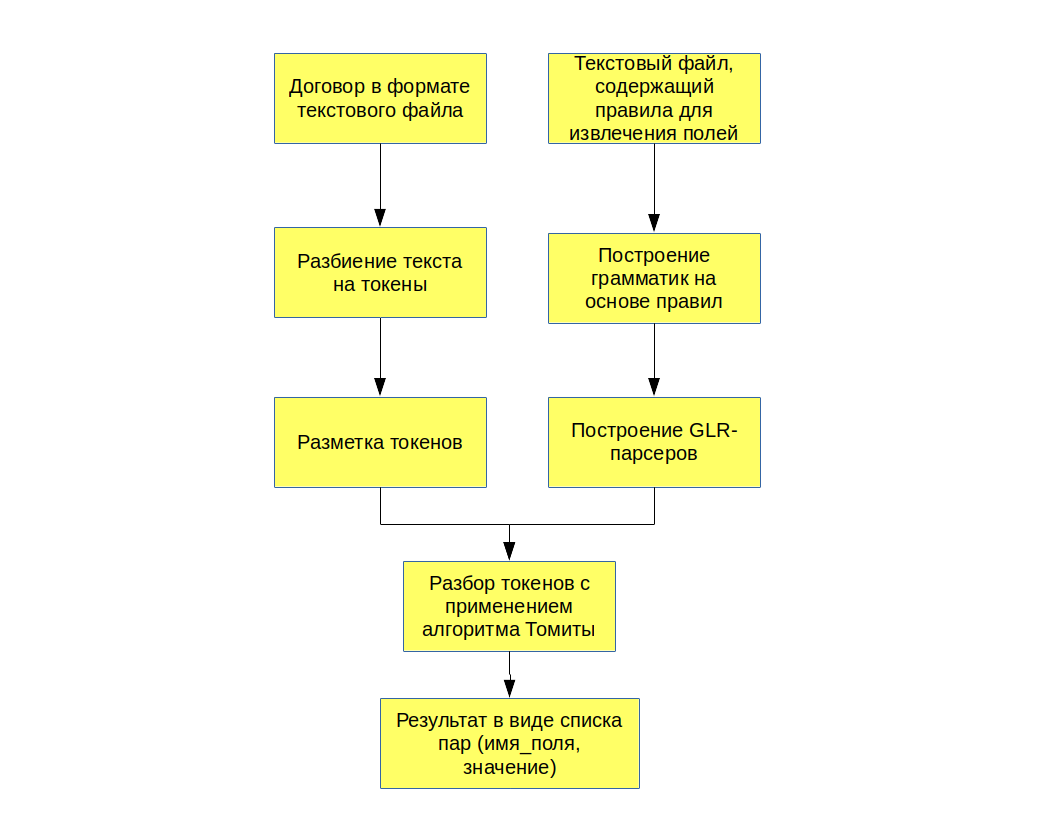
\includegraphics[width=\textwidth]{img/ProjectDiagram.png}
\caption{\label{fig:project-diagram}Схема работы программы}
\label{fig:project-diagram}
\end{figure}

\section{Разбор входного текста}
\subsection{Поддерживаемые форматы}
Документ должен поступать на вход в формате plain text. Предполагается, что файл был получен средствами офисного редактора путем экспортирования документа в формат txt. Для работы именно с такими файлами разрабатывалась и тестировалась та часть программной реализации, которая отвечает за обработку входных текстов. Любые внесенные вручную правки и коррективы могут негативно сказаться на эффективности работы программы.

Основным языком документа должен быть русский. Однако стоит отметить, что текст на других языках будет принят программой и успешно обработан. Более того, если речь идет об английском языке, можно будет даже сформировать набор правил для извлечения определенной информации из такого текста. Однако же это скорее <<побочный эффект>>, нежели самоцель. Реализация нацелена именно на работу с русским языком, и для остальных корректная работа не гарантируется. В лучшем случае будет недоступна часть функционала, в худшем - может призойти что угодно, начиная от ошибки при компиляции правил, и заканчивая аварийным завершением. Связано это главным образом с тем, что при разборе программа в немалой степени опирается на морфологические характеристики слов, и получение таких характеристик реализовано только для русского языка.

На данный момент наилучшая поддержка среди всех типов официальных документов реализована именно для договоров. Для них заготовлено несколько встроенных правил, позволяющих извлекать специфические для этого типа документов поля. Однако же поля, описывающие более общую информаию, такую как имя человека, адрес, теоретически можно извлечь из текстовых файлов произвольного формата, составленных на русском языке, как деловых, так и художественных. При составлении таких правил были учтены различные вариации написания, что позволяет заявлять высокий уровень универсальности.

Для входных файлов поддерживается только формат txt (plain text). В процессе написания программы рассматривался также ряд дополнительных форматов, для которых было бы логично обеспечить поддержку - в первую очередь, это наиболее популярные офисные форматы: DOCX, DOC, ODT. Более того, имелись идеи касательно того, что метаданные этих форматов можно было бы использовать как дополнительный источник информации, позволяющий идентифицировать поле. Например, мы знаем, что номер телефона одного из контрагентов очень часто можно найти в разделе, содержащем слово <<реквизиты>>. Тогда на основе анализа метаданных формата мы могли бы довольно легко получить список разделов, найти среди них нужный, и, получив текст для него текст, искать уже более точечно. При работе с сырым текстом для реализации чего-то подобного приходится уже прибегать к регулярным выражениям, которые предоставляют гораздо меньший уровень надежности анализа. Нет никаких гарантий того, что паттерн, описывающий заголовок раздела, не совпадет с рядовым участком текста.

\subsection{Разбор текста на фрагменты и разметка}
Разбор и разметка входного текста производится в несколько последовательных этапов:
\begin{enumerate}
  \item Разбиение текста на абзацы по символу перехода на новую строку
  \item Каждый абзац разбивается по опредленному набору символов на последовательнсть слов
  \item Для каждого слова производится морфологический анализ и нормализация
\end{enumerate}
В конечном итоге получается массив из упорядоченных последовательностей токенов.

Сущность <<токен>> инкапсулирует слово и совокупность его характеристик.
\begin{ListingEnv}
\begin{Verb}

struct Token {
    // слово, полученное в результате разбиения абзаца
    UnicodeString word;
    // нормализованное слово
    UnicodeString normalForm;
    // часть речи
    UnicodeString partOfSpeech;
    // битовая маска, которая содержит 
    // совокупность морфологических характеристик
    unsigned propMask = 0;
    ...
};
\end{Verb}
\caption{Объявление класса Token}
\label{list:TokenClass}
\end{ListingEnv}
Как можно увидеть из листинга \ref{list:TokenClass}, \lstinline{Token} содержит битовую маску, на которую накладываются его морфологические характеристики. Эта маска формируется из перечисления \lstinline{MorphProperty}. Его объявление показано в листинге \ref{list:MorphProperty}.
\begin{ListingEnv}
\begin{Verb}

enum MorphProperty {
    // имя
    FIRST_NAME = 01,
    // фамилия
    SECOND_NAME = 02,
    // отчество
    PATR = 04,
    // инициал
    INIT = 010,
    // географический объект
    GEOX = 020,
    // число
    NUMB = 040,
    // название месяца
    MONTH = 0100,
    // специальный символ
    NUMERO_SIGN = 0200
};

\end{Verb}
\caption{Объявление перечисления MorphProperty}
\label{list:MorphProperty}
\end{ListingEnv} 

Разметка и преобразование слов в токены происходит в несколько этапов. На первом этапе мы очищаем <<сырые>> слова от лишних символов, включая пробельные символы, знаки пунктуации и кавычки. Очистка происходит в момент разбиения абзаца на отдельные слова.
\begin{Verb}
std::vector<UnicodeString> plainTokens;
// метод формирует паттерн из второго параметра
// вида [s1s2s3...]
// разбивает по нему строку plainSentence
// результат записывает в plainTokens
split_unistring(plainSentence, {"\\s", "\\;", "\\:",
                                "\\,", "\\(", "\\)",
                                "\\<", "\\>", "\\{",
                                "\\}", "\\."
                                }, plainTokens);
\end{Verb}
После этого полученный массив слов передается на вход анализатору. В качестве анализатора была выбрана pymorphy2 - программа для морфологического разбора слов. По заявлениям автором, в программе обеспечена поддержка русского и украинского яызков. Для классификации слов pymorphy2 использует размеченные корпуса проекта OpenCorpora. Кроме того, реализован алгоритм разбора несловарных слов на основе ряда эвристик. 

Ключевой участок функции, реализующей морфологический анализ, показан в листинге \ref{list:MorphAnalysis}. Для каждого слова вызывается метод \lstinline{MorphAnalyzer.parse()}, который возвращает результат в виде массива структур типа \lstinline{Parse} с информацией о том, как слово может быть разобрано. 

\begin{ListingEnv}
\begin{Verb}
// получение массива морфологических характеристик для слова
morph_results = morph.parse(word)
cdef unsigned propMask
for morph_result in morph_results:
    // инициализируем объект, в который
    // будет записываться результат
    analysis_res = make_shared[AnalysisResult]()
    // проверяем, что результат имеем достаточный
    // уровень надежности
    if morph_result.score > 0.1:
        // записываем результат нормализации
        analysis_res.normalForm = morph_result.normalForm
        propMask = 0 
        // в том случае, если определена часть речи
        // запоминаем ее
        if morph_result.tag.POS is not None:
            analysis_res.partOfSpeech = morph_result.tag.POS
        // те же самые проверки для имени
        // отчества, фамилии, инициалов и
        // географического объекта
        if 'Name' in morph_result.tag:
            propMask |= FIRST_NAME
        if 'Patr' in morph_result.tag:
            propMask |= PATR
        if 'Surn' in morph_result.tag:
            propMask |= SECOND_NAME
        if 'Init' in morph_result.tag:
            propMask |= INIT
        if 'Geox' in morph_result.tag:
            propMask |= GEOX
        analysis_res.nameCharMask = propMask
    else:
        // в том случае, если результат недостаточно
        // надежен, записываем в нормальную форму само слово
        // и двигаемся дальше
        analysis_res.normalForm = tok
\end{Verb}
\caption{Морфологический анализ}
\label{list:MorphAnalysis}
\end{ListingEnv}

Мы запоминаем полученные морфологические харакетистики и после этого производим еще несколько дополнительных проверок на предмет соотвествия тем или иным сущностям.
\begin{Verb}
unsigned checkResult = DictChecker.check(currentToken);
if ((checkResult & DictChecker::MatchFlags::MONTH)) {
    currentToken.propMask |= MorphProperty::MONTH;
}
if ((checkResult & DictChecker::MatchFlags::NUMBER)) {
    currentToken.propMask |= MorphProperty::NUMB;
}
if ((checkResult & DictChecker::MatchFlags::COUNTRY)) {
    currentToken.propMask |= MorphProperty::COUNTRY;
}
\end{Verb}
Класс \lstinline{DictChecker} содержик методы для сопоставления слова с рядом заранее определенных регулярных выражений, которые описывают некоторые сущности. К этим сущностям относятся: число, месяц, страна.

После этого мы сохраняем полученный токен и переходим с следующему слову.

\subsection{Особенности работы pyrmorphy2}
Взглянем еше раз на листинг \ref{list:MorphAnalysis}. Рассмотрим поподробнее, что именно представляет собой результат вызова функции \lstinline{MorphAnalyzer.parse()}. 

Как уже было сказано ранее, он возвращает массив объектов \lstinline{Parse}. У каждого объекта типа \lstinline{Parse} есть поле \lstinline{tag}. Тэг содержит набор морфологических характестик для данного слова. Харакетискики берутся из проекта OpenCorpora, равно как и их обозначения. Ниже показан пример содержимого поля \lstinline{tag}.
\begin{Verb}
>>> morph = pymorphy2.MorphAnalyzer()
>>> p = morph.parse('стали')[0]
>>> p.tag
OpencorporaTag('VERB,perf,intr plur,past,indc')
\end{Verb}
В данном случае слово <<стали>> интерпретировалось как глагол ( \lstinline{VERB} ), множественного числа ( \lstinline{plur} ), совершенного вида ( \lstinline{perf} ), прошедшего времени ( \lstinline{past} ).

Также у каждого объекта типа \lstinline{Parse} присутствует поле \lstinline{normal_form}. В нем содержится нормализованный вариант исходного слова.
\begin{Verb}
>>> morph = pymorphy2.MorphAnalyzer()
>>> p = morph.parse('стали')[0]
>>> print(p.normal_form)
стать
\end{Verb}

Поскольку метод \lstinline{MorphAnalyzer.parse()} возвращает массив объектов типа \lstinline{Parse}, бывает необходимо выбрать из них наиболее подходящий. Для этих целей служит поле \lstinline{score}, которое также обозначается как оценка P(tag|word). Данное поле представляет собой оценку вероятности того, что данный разбор правильный. Она высчитывается на оснве корпуса OpenCorpora: ищутся все неоднозначные слова со снятой неоднозначностью, для каждого слова считается, сколько раз ему был сопоставлен данный тег, и на основе этих частот вычисляется условная вероятность тега (с исползованием сглаживания Лапласа). Данная оценка помогает улучшить разбор, но ее зачастую недостаточно для надежного снятия неоднозначности, как минимум по следующим причинам:
\begin{itemize}
  \item то, как нужно разбирать слово, зависит от соседних слов; pymorphy2 работает только на уровне отдельных слов
  \item условная вероятность P(tag|word) оценена на основе сбалансированного набора текстов; в специализированных текстах вероятности могут быть другими - например, возможно, что в металлургических текстах P(NOUN|стали) > P(VERB|стали)
  \item в OpenCorpora у большинства слов неоднозначность пока не снята; выполняя задания на сайте OpenCorpora, можно непосредственно помочь улучшить оценку P(tag|word) и, следовательно, качество работы pymorphy2
\end{itemize}
Массив результатов сортируется по убыванию значения поля \lstinline{score}, поэтому в большинстве случаев бывает достаточно брать первый вариант.

\subsection{Выбор инструмента для разметки текста}
Выбор pymorphy2 обусловился качеством его работы, простотой и относительной легкостью его интеграции в проект. Рассмтривались и другие программы и библиотеки для морфологического разбора слов. Среди них особенно можно выделить MyStem, АОТ, TreeTagger и Stemka. 

MyStem - программа, разработанная в Яндексе, умеет производить анализ несловарных слов и разрешать морфологическую неоднозначность. Именно она используется в <<Томита-парсер>>. Показывает достаточно качественные результаты, однако с ее использованием связан ряд проблем. Во-первых, официально она распространяется только в виде исполняемого файла, поэтому использовать ее внутри программы не всегда удобно. Неофициально она также распространяется в виде библиотеки вместо с <<Томита-парсер>>, однако API для нее никак не задокументирован и не совсем ясны правовые последствия использования данной библиотеки.

АОТ - очень мощная система всестороннего анализа естественного языка. Ее возможности включают не только морфологический, но также графематический, синтаксический и семантический виды анализа. Умеет обрабатывать не только русский, но также английский и немецкий языки. К числу ее недостатков можно отнести коммерческую лицензию.

TreeTagger - инструмент для мофролгической разметки текстов на естественных языках, реализация которого построена на деревьях принятия решений. Поддерживает большое количество языков, включая русский, английский, немецкий, испанский, болгарский, итальянский. TreeTagger, как и MyStem, распространяется в виде исполняемого файла. В списке недостатков относительно невысокое качество разбора и сложность интеграции в проект. К достоинствам можно отнести большое количество поддерживаемых языков и высокую скорость работы.

Stemka - программа для выделения морфологической основы слов русского языка. Работает только со словырными словами. Недостатки: бедный по совеременным меркам функционал и отсутствие признаков активной разработки на протяжении долгого времени.

\section{Описание и реализация языка правил}
\subsection{Общая структура языка}
В рамках данной магистерской диссертации был реализован простой декларативный язык, позволяющий извлекать информационные поля из слабоструктурированных документов. Язык разрабатывался как достаточно простое, функциональное и дружелюбное к пользователю средство взаимодействия с программой.

Каждый файл с правилами должен иметь две основные секции: секцию правил и секцию комманд. Секция правил (возможно, пустая) содержит формальные описания синтаксической и морфологической структуры некоторых сущностей (например, полное имя человека или адрес). Секция комманд содержит указания на то, какие из описанных сущностей нужно искать, в каком порядке и в каком контексте.

Парсер для языка генерировался при помощи YACC GNU Bison. В качестве лексического анализатора испольщовался GNU Flex. Было решено использовать YACC в первую очередь в виду простоты описания грамматики языка, ее изменения и расширения. Парсер генерируется на языке C++.

\subsection{Секция правил}
Секция правил задается ключевым слово \lstinline{%rules} содержит формальные описания языковой структуры для искомых информационных полей (или их составляющих). Ниже можно видеть примеры таких правил.
\begin{Verb}
PassportSeries = num(len: 4);
PassportNumber = num(len: 6);
Address = Town Street;
RentPeriodStart = "с" FullDate;
RentPeriodEnd = "по" FullDate;
RentPeriod = "с" FullDate "по" FullDate;
EmployerName = "наниматель";
OwnerName = "наймодатель";
Requisits = "реквизит";
\end{Verb}

Опишем базовые понятия, которые используются при описании правил.
\begin{description}
  \item[Терминальное слово] Описывает некоторое слово естественного языка, обладающее некоторыми характеристиками. Существует определенный набор заранее заданых слов, который базируется на характеристиках, получемых от анализатора pymorphy2. Среди них:
  \begin{description}
    \item [name] имя человека, например, Борис или Наталья.
    \item [surn] фамилия человека (срабатывает на довольно узком наборе фамилий, как правило имеющих окончание -ов).
    \item [patr] отчество.
    \item [init] инициал (по сути, однобуквунное слово с большой буквы, оканчивающееся точкой). Плохо распознается через pymorphy2, по этому реализована дополнительная проверка с помощью регулярного выражения.
    \item [word] абсолютно любое слово. Злоупотребление данным терминальным символом может привести к замедлению работы программы.
    \item [num] число.
    \item [month] название месяца.
    \item [geox] географический объект. Сюда входят: страны, города, континенты, названия морей, озер, рек, гор (все, что попадает под определение топонима).
    \item [adjf] прилагательное полное
    \item [adjs] прилагательное краткое
    \item [advb] наречие
    \item [comp] сравнительная форма
    \item [conj] союз
    \item [grnd] деепричастие
    \item [infn] глагол (инфинитив)
    \item [intj] междометие
    \item [noun] имя существительное
    \item [npro] местоимение (сущ)
    \item [numr] числительное
    \item [prcl] частица
    \item [prep] предлог
    \item [prtf] причастие полное
    \item [prts] причастие краткое
    \item [verb] глагол (лич форма)
    \item [empty] пустой терминал
  \end{description}
  \item[Нетерминальное слово или правило] Является само по себе правилом, описывающим некую сущность. На него накладываются следующие ограничения: должно быть определено в секции правил либо должно принадлежать множеству встроенных правил, которые определяются заранее внутри программы. В программе определены следующие встроенные правила (реализация в листинге \ref{list:StandardRules}):
  \begin{description}
    \item[WordSeq] произвольная последовательность слов, возможно пустая.
    \item[PersonFullName] имя человека, включающее указание фамилии, имени и отчества.
    \item[FullDate] дата в формате <<число месяц год>>.
    \item[ApartmentNumber] номер квартиры.
    \item[Town] город.
    \item[Street] улица.
  \end{description}
  \item[Предикат] условие, применяемое к терминальному слову. Реализована поддержка следующих предикатов:
  \begin{description}
    \item[upper1] слово должно начинаться с большой буквы.
    \item[regex] слово должно удовлетворять указанному паттерну регулярного выражения.
    \item[len] слово должно быть указанной длины в символах.
    \item[quoted] слово должно быть заключено в кавычки.
  \end{description}
\end{description}

\begin{ListingEnv}
\begin{Verb}
// реализация правила WordSeq
WordSeq = empty;
WordSeq = word;
WordSeq = WordSeq word;

// реализация правила PersonFullName
// предполагается порядок Фам Имя Отч
// исходя из изученных примеров документов
PersonFullName = Surname SecPart;
SecPart = FullRec | ShordRec;
FullRec = name patr;
ShortRec = init init;
Surname = surn | word(predicates: upper1);

// реализация правила FullDate
YearSuffix = "г" | "год" | empty;
Day = num(len: 1..2)
Year = num(len: 4)
FullDate = Day Month Year YearSuffix;

// реализация правила ApartemntNumber
ApartmentPrefix = "кв" | "квартира" | empty;
NumSign = num_sign | empty;
ApartmentNumber = ApartmentPrefix num_sign num(len: 1..3);

// реализация правила Town
TownPrefix = "город" | "г" | empty;
Town = TownPrefix geox;

// реализация правила Street
StreetPrefix = "ул" | "улица";
StreetPrefix = "бул" | "бульва";
StreetPrefix = "просп" | "проспект";
StreetPrefix = "пер" | "переулок";
HousePrefix = "д" | "дом" | empty;
StreetName = word(predicates: upper1);
Street = StreetPrefix StreetName HousePrefix num(len: 1..3); 
\end{Verb}
\caption{Реализация встроенных правил}
\label{list:StandardRules}
\end{ListingEnv}

Грамматика для языка правил описывалась при помощи YACC GNU Bison. Ниже описание грамматики для правила.
\begin{Verb}
rule_list
    : %empty
    | rule_list rule
    ;
/* SEMICOLON - точка с запятой */
rule 
    : complex_rule SEMICOLON
    ;
/* CAPITAL_WORD - слово на латинице */
/* начинающееся с большой буквы */
/* ASSIGN - знак равно */
simple_rule
    : CAPITAL_WORD ASSIGN rhs_chain
    ;
/* DELIM - вертикальная черта */
complex_rule
    : simple_rule
    | complex_rule DELIM rhs_chain
    ;
\end{Verb}
Правило записывается как $Rule = rhs\_chain_1 | rhs\_chain_2 | \dots | rhs\_chain_n$, где $Rule$ - имя правила, $rhs\_chain_i$ - произвольная последовательность терминальных и нетерминальных слов, возможно с предикатами. Ниже приведены примеры правил.
\begin{Verb}
//примеры simple_rule
Surname = surn;
Surname = word(upper1);
Address = Town Street;
PassportSeries = num(len: 4);
//пример complex_rule
//по сути альтернативная запись
//первых двух правил
Surname = surn | word(upper1);
\end{Verb}
Далее приведена грамматика для конструкции rhs\_chain.
\begin{Verb}
rhs_chain
    : labeled_rhs_term
    | rhs_chain labeled_rhs_term
    | labeled_rhs_nterm
    | rhs_chain labeled_rhs_nterm
    | rhs_term_empty
    ;
\end{Verb}
Как видно из грамматики, rhs\_chain явялется произвольной последовательностью сущностей labeled\_rhs\_term, labeled\_rhs\_nterm и rhs\_term\_empty. Первая представляет собой произвольную последовательность <<помеченных>> терминальных слов, другими словами - таких терминальных слов, на которые могут быть наложены дополнительные ограничения в виде предикатов. Грамматика описана в листинге \ref{list:LabeledRhsTerm}.
\begin{ListingEnv}
\begin{Verb}
// DOUBLE_QUOTE - двойная кавычка (")
// WORD - любое слово с маленькой буквы
rhs_term
    : WORD
    | DOUBLE_QUOTE WORD DOUBLE_QUOTE
    ;
// EMPTY_WORD - ключевое слово empty
rhs_term_empty
    : EMPTY_WORD
    ;
// LBRACKET, RBRACKET - круглые скобки, левая и правая
// NUM_TERM - ключевое слово num
// обозначающее терминальное слово, соотвествующее числу
labeled_rhs_term
    : rhs_term
    | rhs_term LBRACKET prop_list length_info regex RBRACKET
    | NUM_TERM
    | NUM_TERM LBRACKET prop_list length_info regex RBRACKET
    ;
\end{Verb}
\caption{Грамматика для описания терминального слова в правой части правила}
\label{list:LabeledRhsTerm}
\end{ListingEnv}
Cущность rhs\_term\_empty представляет собой специальное обозначение <<пустого>> терминального слова. Она вынесена в отдельное правило, так как было решено наложить на нее дополнительное ограничение: $empty \in rhs\_chain \rightarrow |rhs\_chain| = 1$. Иначе говоря, если последовательность символов в правой части включает в себя пустой терминал, то он должен быть единственным элементом этой последовательности.

Сущность \lstinline{prop_list} представляет собой секцию описания предикатов. Она должна располагаться в круглых скобках после указания имени терминального слова.
\begin{Verb}
// PROPS_SECT - predicates (название секции предикатов)
// COLON - символ двоеточия
// COMMA - запятая
prop_list
    : %empty
    | PROPS_SECT COLON prop
    | prop_list COMMA prop
    ;
prop
    : simple_prop
    ;
// PROP_START_UPPER_TOK - предикат upper1
simple_prop
    : PROP_START_UPPER_TOK
    ;
\end{Verb}
Предиакты перечисляются после объявления секции через запятую.

В листинге \ref{list:LabeledRhsTerm} фигурирует сущность \lstinline{length_info}. Данная сущноcть описывает конструкция предиката \lstinline{length}. Этот предикат позволяет накладывать ограничения на длину слова.
\begin{Verb}
// LENGTH_SECT - название секции length (len)
// NUM - число
// ELLIPSIS - две точки (..)
length_info
    : %empty
    | LENGTH_SECT COLON NUM
    | LENGTH_SECT COLON NUM ELLIPSIS NUM
    ;
\end{Verb}
Можно указывать как точную длину, так и нижнюю и верхнюю границы.

Далее рассмотрим еще один особый случай предиката - предикат \lstinline{regex}. Он позволяет задавать ограничение с помощью паттерна регулярного выражения, тем самым определяя допустимое множество слов.
\begin{Verb}
// REGEX_SECT - название секции (regex)
regex
    : %empty
    | REGEX_SECT COLON REGEX_PATTERN
    ;
\end{Verb}

Сущность \lstinline{labeled_rhs_nterm} представляет собой описание синтаксиса правила, которое может встретиться в правой части другого правила. Префикс \lstinline{labeled} в данном случае может ввести в заблуждение, посколько сущности \lstinline{rhs_nterm} на данный момент не поддерживают задание ограничений в виде предикатов. Изначально планировалась поддержка некоторых предикатов (по очевидным причинам не всех, так как правило, в отличие от терминального слова, не обязательно соотвествует одному токену), но из-за ряда технических сложностей пока что было решено от нее отказаться.
\begin{Verb}
rhs_nterm
    : CAPITAL_WORD
    | PERSON_NAME
    | AGREEMENT_DATE
    | FULL_DATE
    | APARTMENT_NUM
    | WORD_SEQUENCE
    | TOWN
    | STREET
    ;

labeled_rhs_nterm
    : rhs_nterm
    ;
\end{Verb}
Как видим, сущность \lstinline{rhs_nterm} включает также ряд заранее определенных нетерминыльных слов для встроенных правил, определения для которых приводились в листинге \ref{list:StandardRules}.

\subsection{Секция команд}
В секции команд перечисляются сущности, которые нужно искать, их контекст и зависимости. Ниже можно видеть пример оформления секции команд.
\begin{Verb}
%commands
Find FullDate (hint_words: "выдавать", "когда") 
with deps (upper: Requisits, OwnerName) 
as RegistrationDate;

Find FullDate with deps (left: Town) as AgreementDateValue;
\end{Verb}
Секция команд не может быть пустой. Она начинается с ключевого слова \lstinline{%commands}. Далее, разделенные точкой с запятой, следуют команды \lstinline{Find}. Синтаксис команды \lstinline{Find} описан в качестве грамматики для GNU Bison.
\begin{Verb}
// FIND - ключевое слово Find
command_find
    : FIND rhs_nterm
    ;
\end{Verb}
Это самый базовый вариант записи команды, в которой указывается правило, соотвествия для которого мы должны искать. На правило, указанное в рамках команды, накладываются следующие ограничения:
\begin{enumerate}
  \item Оно должно быть определено в секции правил
  \item Или же оно должно принадлежать множеству встроенных правил, определения для которых представлены в листинге \ref{list:StandardRules}.
\end{enumerate}

Базовый вариант записи команды может расширен для указания дополнительных параметров, таких как: слова из контекста или \lstinline{hint_words}, зависимости и псевдоним.
\begin{ListingEnv}
\begin{Verb}
closed_hw_list
    : LBRACKET hint_word_list RBRACKET
    ;
command
    : command_find dep_part alias SEMICOLON
    | command_find closed_hw_list dep_part alias SEMICOLON
    ;
\end{Verb}
\caption{Расширенный синтаксис команды Find}
\label{list:FindExtSyntax}
\end{ListingEnv}

Сущность \lstinline{hint_word_list} представляет собой список слов, которые могут встретиться в некотором радиусе от искомой конструкции, которую описывает правило. Приведем пример нахождения поля <<Наниматель>>.
\begin{myexample}
\label{examp:HintWodsExamp}
Гражданин Иванов Иван Иванович, паспорт (серия, номер, выдан) 6545 033655, именуемый в дальнейшем "Наймодатель", с одной стороны, и гражданин Петров Петр Петрович, паспорт (серия, номер, выдан) 6565 033654, именуемый в дальнейшем "Наниматель", с другой стороны, именуемые в дальнейшем «Стороны», заключили настоящий договор, в дальнейшем «Договор», о нижеследующем:
\end{myexample}
\begin{ListingEnv}
\begin{Verb}
%rules
Employer = PersonFullName WordSeq "наниматель";
%commands
Find Employer;
\end{Verb}
\label{list:EmployerExampleRules}
\caption{Правила для нахождения полного имени человека}
\end{ListingEnv}

Допустим, у нас есть договор, содержащий текст из примера \ref{examp:HintWodsExamp}. Также предположим, что у нас есть набор правил из листинга \ref{list:EmployerExampleRules}. Как мы уже видели в листинге \ref{list:StandardRules}, правило \lstinline{PersonFullName} определяет такую сущность как <<полное имя человека в формате Фамилия Имя Отчество>>. На основании неких эмпирических наблюдений и здравого смысла мы предпологаем, что имя представителя контрагента <<Наниматель>> будет зафиксировано в договоре в непосредственной близости от слова <<наниматель>>, и что это слово встретится позже по тексту. Однако же, запустив программу на тексте из примера \ref{examp:HintWodsExamp} и подав на вход правила из листинга \ref{list:EmployerExampleRules}, мы получим следуующий результат:
\begin{Verb}
Field: Employer, Value: Иванов Иван Иванович
Field: Employer, Value: Петров Петр Петрович
\end{Verb}
Результат, хоть и несколько не такой, как мы ожидали, однако же вполне закономерный. Программа разбирает текст документа на уровне абзаца, поэтому областью действия описанных пользовательских правил является также абзац. В листинге \ref{list:EmployerExampleRules} описано то, что словами можно выразить так: найти полное имя человека, такое что после него по тексту в том же абзаце встретится слово <<наниматель>>. Поскольку весь текст из примера \ref{examp:HintWodsExamp} располагается в одном абзаце, то вполне логичен и результат: <<Иванов Иван Иванович>> и <<Петров Петр Петрович>> удовлетворяют сформированному запросу.

Теперь немного модифицируем команду \lstinline{Find} из примера \ref{examp:HintWodsExamp}, записав ее так, как показано в листинге \ref{list:EnhancedEmployerRules}.
\begin{ListingEnv}
\begin{Verb}

Find PersonFullName(hint_words: "наниматель");
\end{Verb}
\caption{Поиск нанимателя с использованием hint\_words}
\label{list:EnhancedEmployerRules}
\end{ListingEnv}
Как видно, в описании команды появилась дополнительная секция \lstinline{hint_words}. В данной секции перечисляются слова, которые мы ожидаем найти в непосредственной близости от искомой сущности. Можно сформулировать по другому: такие слова, которые характеризуют искомую сущность. В случае с официальными документами характеризующие слова очень часто располагаются рядом с теми сущностями, которые они характеризуют. Например, если в договоре встречается телефонный номер, то очень высока вероятность того, что где-то поблизости указано на то, что это именно телефонный номер, а также на то, кому он принадлежит. Секция \lstinline{hint_words} позволяет указать ряд ключевых слов и тем самым отсечь часть нерелевантных совпадений. На принадлежность ко множеству \lstinline{hint_words} проверяются все слова, которые находятся в непосредственной близости от найденной сущности. <<В непосредственной близости>> в данном случае стоит трактовать как <<в том же самом абзаце>>. Для каждого совпадения на основе \lstinline{hint_words} высчитывается эвристика, величина которой прямо пропорциональна количеству наденных слов из \lstinline{hint_words} и обратно пропорциональна суммарному расстоянию от подстроки, соотвествующей совпадению, до наденного ключевого слова. Дадим определение расстоянию.
\begin{mydefinition}
Пусть $w_1 w_2 \dots w_n$ - все слова из текущего рассматриваемого абзаца для некоторого документа, поданого на разбор. Пусть  $W = w_i \dots w_j$ - результат разбора данного абзаца для некоторого правила $S$, причем $1 \leq i < j \leq n$. Тогда определим $Dist(W, w_k) = \min(|i - k|, |j - k|) \iff (1 \leq k < i) \lor (j > k \geq n)$.
\end{mydefinition}
Таким образом, на основе эвристики мы будет отсеивать результаты по признаку наибольшего соответствия заданному контексту. Если возникнет ситуация, при которой нескольким результатам разбора будет соответствовать одна и та же наилучшая эвристика, тогда все эти результаты будут истрактованы как верные.

Итак, если мы изменим команду \lstinline{Find} в листинге \ref{list:EmployerExampleRules} на модифицированную команду из листинга \ref{list:EnhancedEmployerRules}, и запустим программу, то получим следующий результат:
\begin{Verb}
Field: Employer, Value: Петров Петр Петрович
\end{Verb}
Это как раз тот результат, который нас полностью устроит.

Если мы взглянем на листинг \ref{list:FindExtSyntax}, то увидим, что расширенный синтаксис команды \lstinline{Find} также содержит сущность \lstinline{dep_part}, которая позволяет указывать зависисмости для искомого правила. Синтаксис описания зависисмостей можно описать следующей схемой:
\begin{Verb}
ledd
    : left_deps_descr
    ;
rdd
    : right_deps_descr
    ;
udd
    : upper_deps_descr
    ;
lodd
    : lower_deps_descr
    ;
dep_part
    : WITH DEPS LBRACKET ledd rdd udd lodd RBRACKET
    | %empty
    ;
\end{Verb}
Зависимости классифицируются по пространственному признаку: 
\begin{itemize}
  \item Левые зависимости (или предшествующие искомой сущности в рамках текущего абзаца)
  \item Правые зависимости (или опережающие в рамках, опять же, абзаца)
  \item Верхние зависимости (или предшествующие в рамках всего текста)
  \item Нижние зависимости (или опережающие в рамках всего текста)
\end{itemize}

Рассмотрим грамматику, описывающую \lstinline{left_deps_descr}.
\begin{Verb}
// LEFT_DRPS_SECT - название секции левых зависимостей (left)
left_deps_descr
    : LEFT_DEPS_SECT COLON rhs_nterm
    | left_deps_descr rhs_nterm
    | %empty
    ;
\end{Verb}
\lstinline{right_deps_descr}, \lstinline{upper_deps_descr} и \lstinline{lower_deps_descr} описываются по аналогии. Как видно из листинга, описание зависимости включает в себя список нетерминальных слов (или, другими словами, правил). Таким образом, когда мы указывем некое правило как зависимость, мы ожидаем, что сущность, которую оно описывает, встретится, соответственно, ниже, выше, левее или правее по тексту от зависимой сущности. Приведем пример.
\begin{myexample}
Договор найма жилого помещения № 1122\newline
г. Ростов-на-Дону «19» августа 2015 г.\newline
Гражданин Иванов Иван Иванович, паспорт (серия, номер, выдан) 6545 033655, именуемый в дальнейшем "Наймодатель", с одной стороны, и гражданин Петров Петр Петрович, паспорт (серия, номер, выдан) 6565 033654, именуемый в дальнейшем "Наниматель", с другой стороны, именуемые в дальнейшем «Стороны», заключили настоящий договор, в дальнейшем «Договор», о нижеследующем: 
\label{examp:Dependencies}
\end{myexample}
В тексте из примера \ref{examp:Dependencies} приведен отрывок, который включает в себя первые три абзаца договора о найме жилого помещения: абзац с номером догвора, абзац с местом и датой заключения договора и, наконец, абзац с информацией о контрагентах. Допустим, что мы хотим извлечь поле, содержащее дату заключения договора. Попытаемся сделать это с помощью правил из листинга \ref{list:AgrDate}.
\begin{ListingEnv}
\begin{Verb}
%rules
AgreementDate = FullDate;
AgreementDateInContext = Town AgreementDate;
%commands
Find AgreementDateInContext;
\end{Verb}
\caption{Правила извлечения даты заключения договора}
\label{list:AgrDate}
\end{ListingEnv}
Результат работы программы на входных данных из примера \ref{examp:Dependencies} и листинга \ref{list:AgrDate} будет следующим:
\begin{Verb}
Extraction result:
Field name: AgreementDateInContext
Field value: г Ростов-на-Дону 19 августа 2015
\end{Verb}
Как видно, результат в целом правильный, но содержит лишнюю информацию. В листинге \ref{list:AgrDate} при описании правила \lstinline{AgreementDateInContext} мы указали, что дата заключения договора, как правило, непосредственно соседствует с названием города, в котором договор был заключен. Побочным эффектом стал вывод лишней информации, посколько искать мы можем только правило целиком. Кроме того, критерий поиска довольно ненадежный, так как есть ненулевая вероятность того, что где-то по тексту договора встретятся другие участки, удовлетворяющие правилу \lstinline{AgreementDateInContext}. Для решения этой проблемы можно воспользоваться инструментом описания зависимостей. Основное его применение - уточнение позиции информационного поля в рамках текста договора относительно других информационных полей или каких-либо иных сущностей, которые можно описать правилами. Как видно по примеру \ref{examp:Dependencies}, дата заключения довора расположена после заголовка с номером договора и до описания контрагентов. Кроме того, как уже было подмечено ранее, с датой, как правило, соседствует название города, в которым был заключен договор. Новый набор правил, отражающий все эти наблюдения, представлен в листинге \ref{list:AgrDateDep}.
\begin{ListingEnv}
\begin{Verb}
%rules
AgreementNum = "договор" WordSeq num_sign num;
Employer = PersonFullName WordSeq "наниматель";
Owner = PersonFullName WordSeq "наймодатель";
%commands
Find FullDate 
with deps (left: Town, 
           upper: AgreementNum, 
           lower: Employer, Owner)
as AgreementDate;
\end{Verb}
\caption{Правила для извлечения даты заключения договора с использованием зависимостей}
\label{list:AgrDateDep}
\end{ListingEnv}
На входных данных из примера \ref{examp:Dependencies} и листинга \ref{list:AgrDateDep} мы получим следующий результат работы программы:
\begin{Verb}
Extraction result:
Field name: AgreementDate
Field value: 19 августа 2015
\end{Verb}
Как раз тот результат, который мы ожиадли.

\subsection{Детали реализации}
Как уже было сказано ранее, разбор пользовательских правил производится с использованием YACC GNU Bison и лексического анализатора GNU Flex. В программе процессом разбора управляет класс \lstinline{GParserDriver}. Он выполняет следующие функции:
\begin{itemize}
  \item Запуск процесса разбора
  \item Обработка ошибок в процессе разбора
  \item Формирование и поддержка в актуальном состоянии ряда служебных структур данных, содержащих информацию о процессе разбора
  \item Хранение результатов разбора
\end{itemize}

\subsection{Реализация разбора секции правил}
Данная секция содержит пользовательские правила в формате $Rule = rhs\_chain_1 | rhs\_chain_2 | \dots | rhs\_chain_n$. Как мы помним, $rhs_chain_i$ - это произвольная последовательность терминальных и нетерминальных слов, возможно с предикатами. Поскольку GNU Bison генерирует парсер, производящий разбор <<снизу вверх>>, то анализ пользовательского правила включает в себя следующие этапы:
\begin{enumerate}
  \item Свертка и накопление предикатов (если есть)
  \item Свертка терминальных и нетерминальных слов, формирование объектов соотвествующих классов с учетом накомпленных предикатов, добавление объектов в коллекцию уже существующих в рамках текущей $rhs\_chain$
  \item Свертка $rhs\_chain$, формирование объекта соотвествующего класса для $Rule$ (если еще не сформирован), сохранение объектов из $rhs\_chain$ в текущий $Rule$
  \item Свертка $Rule$, сохранение соответствующего объекта в списке определенных правил
\end{enumerate}
Предикаты сохраняются в объекты класса \lstinline{Predicate}.
\begin{Verb}
class Predicate {
protected:
    virtual bool equals(const PredicatePtr &other) const = 0;
public:
    virtual ~Predicate() = default;
    virtual bool operator()(const Token &token) = 0;
    virtual unsigned long hash() const = 0;
    ...
};
\end{Verb}
Это абстрактный класс, от которого наследуются классы, реализующие конкретные предикаты. Основным методом в этом классе является \lstinline{bool operator()(const Token &token)}. Эта функция принимает на вход объект класс \lstinline{Token} и возвращает истину в том случае, если токен удовлетворяет телу данного предиката. На данный момент реализована 3 вида предикатов:
\begin{itemize}
  \item \lstinline{UpperCaseFirstPredicate}
  \item \lstinline{RegexPredicate}
  \item \lstinline{LengthPredicate}
\end{itemize}

\lstinline{UpperCaseFirstPredicate} возвращает истину в том случае, если поле \lstinline{word} (листинг \ref{list:TokenClass}) поданного на вход токена начинается с большой буквы. Реализация функции \lstinline{bool operator()(const Token &token)} тривиальна:
\begin{Verb}
bool UpperCaseFirstPredicate::operator()(const Token &token) {
    if (token.word.isEmpty()) {
        return false;
    }
    // извлечение первого символа слова
    auto firstChar = token.word.tempSubString(0, 1);
    // преобразование его в верхний регистр
    // сравнение со сторым значением
    return firstChar.toUpper() == token.word.tempSubString(0,1);
}
\end{Verb}

\lstinline{RegexPredicate} возвращает истину тогда и только тогда, когда поле \lstinline{word} поданного на вход токена удовлетворяет регулярному выражению, хранящемуся в теле класса \lstinline{RegexPredicate}. Регулярное выражение формируется в конструкторе, который принимает на вход строковый паттерн:
\begin{Verb}
RegexPredicate::RegexPredicate(const UnicodeString &pattern) {
    UErrorCode status = U_ZERO_ERROR;
    // создание реглярного выражения из паттерна и
    // сохранение его в поле класса
    regex = std::make_shared<RegexMatcher>(pattern, 0, status);
    if (U_FAILURE(status)) {
        std::ostringstream os;
        os << "Failed to init regex from pattern " << pattern;
        throw std::runtime_error(os.str());
    }
}
\end{Verb}
В функции \lstinline{bool operator()(const Token &token)} осуществляется проверка токена на соответствие регулярному выражению:
\begin{Verb}
bool RegexPredicate::operator()(const Token &token) {
    if (token.word.isEmpty()) {
        return false;
    }
    // устанавливаем token.word в качестве
    // теущего проверяемого слова
    regex->reset(token.word);

    UErrorCode status = U_ZERO_ERROR;
    // осуществляем проверку на соотвествие всему слову
    UBool result = regex->matches(status);
    if (U_FAILURE(status)) {
        return false;
    }
    return result;
}
\end{Verb}

\lstinline{LengthPredicate} возвращает истину в том случае, если длина поля \lstinline{word} входного токена удовлетворяет минимальному и максимальному порогам, хранящимся в теле класса. Для \lstinline{LengthPredicate} определено два конструктора: первый задает ограничение в виде точного значение, а второй - в виде максимального и минимального порога.
\begin{Verb}
// на вход подается единственное значение length
// которым инициализируются минимальный и
// максимальный пороги
LengthPredicate(int length):
    minLength { length },
    maxLength { length } {}
// здесь на вход поступает интервал
LengthPredicate(int minLength, int maxLength):
    minLength { minLength },
    maxLength { maxLength } {}
\end{Verb}
В функции \lstinline{bool operator()(const Token &token)} осуществляется проверка токена на соответствие значениям границ:
\begin{Verb}
bool LengthPredicate::operator()(const Token &token) {
    return token.word.length() >= minLength && 
            token.word.length() <= maxLength;
}
\end{Verb}

При разборе секции правил предикаты хранятся в виде массива объектов \lstinline{Predicate}. При свертке предиката в зависимости от его типа (листинг \ref{list:LabeledRhsTerm}) формируется объект соответствующего класс и добавляется в массив.

Терминальные и нетерминальные слова сохраняются в объекты типа \lstinline{GRuleWord}.
\begin{Verb}
class GRuleWord {
private:
    std::vector<ParentInfo> parentNterms;
    std::vector<ChildWords> childWords;
protected:
    UnicodeString rawValue;
public:
    GRuleWord(const UnicodeString &word);
    GRuleWord(UnicodeString &&word);
    ...
};
\end{Verb}
Это абстрактный класс, от которого наследуются классы \lstinline{Terminal} и \lstinline{NonTerminal}. Класс \lstinline{Teminal} соответствует терминальному слову и содержит ряд дополнительных полей и методов.
\begin{Verb}
class Terminal final: public GRuleWord {
private:
    std::vector<PredicatePtr> predicates;
    ...
public:
    ...
    bool checkToken(const Token&, const UnicodeString & word);
    unsigned getPredciatesSize();
    ...
};
\end{Verb}
Класс \lstinline{Terminal} хранит в себе массив предикатов \lstinline{predicates}, а также содержит служебные методы для работы с предикатами: \lstinline{checkToken} и \lstinline{getPredicatesSize}.
\begin{Verb}
bool Terminal::checkToken(const Token &token, 
                          const UnicodeString &word) const 
{
    if (this->rawValue != word) {
        return false;
    }
    for(const auto &pred : predicates) {
        if (!pred->operator()(token)) {
            return false;
        }
    }
    return true;
}
\end{Verb}
Метод \lstinline{checkToken} используется для проверки того, соответствует ли входной токен терминальному слову. При этом учитываются все предикаты, ассоциированные с данным терминалом. \lstinline{getPredicatesSize} просто возвращает количество хранимых предикатов.

Класс \lstinline{NonTerminal} соответствует нетерминальному слову и связанному с ним правилу.
\begin{Verb}
class NonTerminal final: public GRuleWord {
protected:
    std::vector<ChildWords> childWords;
    ...
};
\end{Verb}
Он дополнительно содержит поле \lstinline{childWords}, которое является массивом объектов, которые в грамматике обозначены как \lstinline{rhs_chain} - произвольные последовательности терминальных и нетерминальных слов. Посмотрим на опредление \lstinline{ChildWords}.
\begin{Verb}
using GRuleWordPtr = std::shared_ptr<GRuleWord>;
using ChildWords = std::vector<GRuleWordPtr>;
\end{Verb}
Как видно, \lstinline{ChildWords} представляет собой массив указателей на объекты типа \lstinline{GRuleWord}. Таким образом, это и есть <<произвольная последовательности терминальных и нетерминальных слов>>.

\lstinline{GRuleWord} является полиморфной сущностью, которая может соответствовать как терминальному, так и нетерминальному слову. Правила хранятся в виде ориентированного графа, где вершинами выступают объекты класса \lstinline{GRuleWord}. Каждая вершина характеризуется следующими свойствами:
\begin{itemize}
  \item Имя вершины - поле \lstinline{rawValue}
  \item Список родительских вершин - поле \lstinline{parentNterms}
  \item В случае, если вершина соответствует нетерминальному слову: массив дочерних вершин - \lstinline{childWords}, организованный в виде массива \lstinline{rhs_chain}, где \lstinline{rhs_chain}, в свою очередь, является массивом объектов типа \lstinline{GRuleWord}
\end{itemize}
Пример графа, иллюстрирующего связи между терминальными и нетерминальными словами в стандартном правиле \lstinline{FullDate} (листинг \ref{list:StandardRules}) можно видеть на рисунке \ref{fig:FullDateRule}. Здесь вершиной корневой вершиной выступает объект класса \lstinline{GRuleWord}, который соответствует нетерминальному слову \lstinline{FullDate}. От него выходят дуги к дочерним узлам, соответствующим терминальным и нетерминальным словам, которые встречаются в правой части правила \lstinline{FullDate} либо его дочерних правил.
\begin{figure}% p означает, что нужно выделить для рисунка
% отдельную страницу; применяется для больших рисунков
\centering
%Здесь могла быть ваша лягушка.
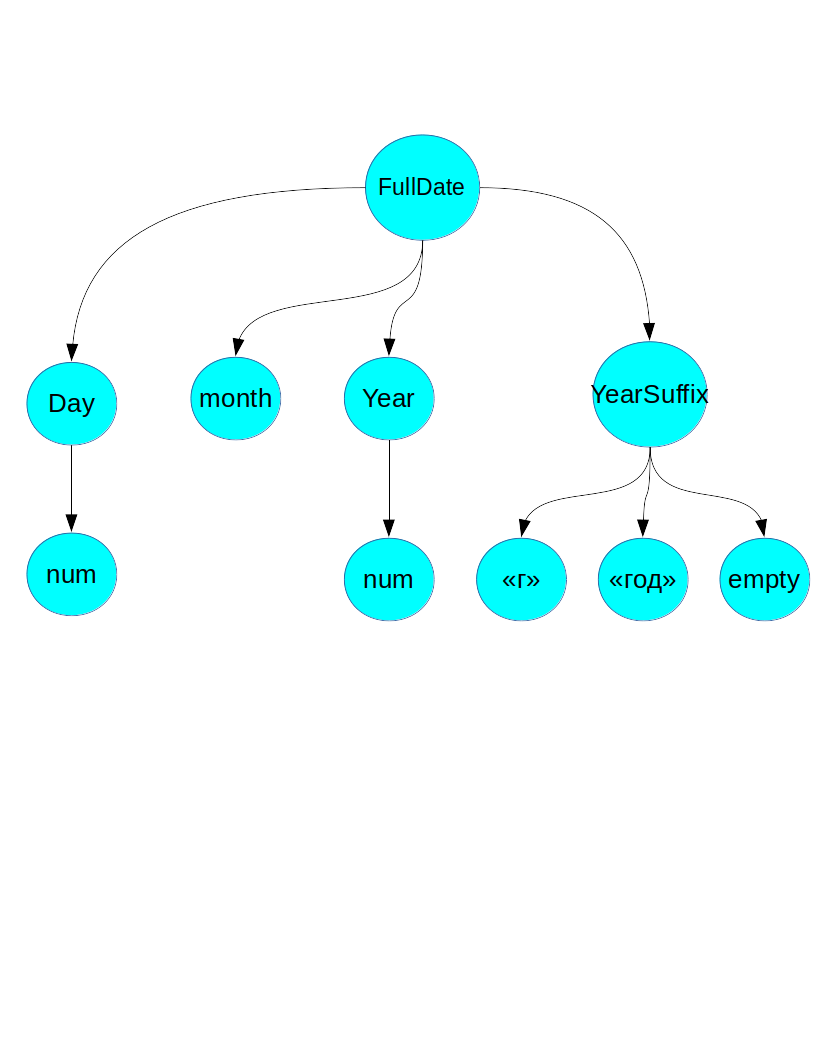
\includegraphics[width=\textwidth]{img/FullDateRule.png}
\caption{Граф отношения терминальных и нетерминальных слов в правиле FullDate}
\label{fig:FullDateRule}
\end{figure}

Теперь посмотрим, как происходит свертка терминальных и нетерминальных слов при разборе секции правил. Сначала рассмотрим случай с терминальным словом. За это отвечает метод \lstinline{handleTermReduction} в классе \lstinline{GParserDriver}.
\begin{Verb}
using PredArray = std::vector<PredicatePtr>;
GRuleWordPtr handleTermReduction(UnicodeString &&rawValue);
GRuleWordPtr handleTermReduction(UnicodeString &&rawValue, 
                                 PredArray &&predicates);
\end{Verb}
Как видно, есть две перегрузки этого метода: первая генерирует терминальное слово лишь на основе его имени, а вторая также обрабатывает список предикатов, связанных с терминалом. Посмотрим на реализацию второй перегрузки.
\begin{Verb}
GRuleWordPtr 
GParserDriver::handleTermReduction(UnicodeString &&rawValue, 
                                   PredArray &&predicates) 
{
    // получение терминала из пула
    auto term = GWordStorage::getTerminal(rawValue, predicates);
    // проверяем, не был ли он определен ранее
    auto termFound = terminals.find(term);
    if (termFound != terminals.end()) {
        return (*termFound);
    } else {
        terminals.insert(term);
        return term;
    }
}
\end{Verb}
Метод берет терминальное слово, соответствующее входному имени и набору предикатов, из специального пула, и затем проверяет, не был ли данный терминал определен ранее. Пул терминальных и нетерминальных слов был организован с целью упростить процедуру сравнения объектов класса \lstinline{GRuleWord}. Так как объекты полиморфные, то практически каждое сравнение предполагало интенсивное использование механизма RTTI (Run-Time Type Information), в частности, функции \lstinline{dynamic_cast}, что могло повлечь за собой негативное влияние на производительность, учитывая, что объекты типа \lstinline{GRuleWord} в программе очень часто сравниваются друг с другом на равенство. В конечном итоге было решено хранить указатели на эти объекты и сравнивать адреса. Благодаря этому сравнения с использованием RTTI производятся только на этапе разбора пользовательских правил. В дальнейшем на этапе поиска информационных полей сравниваются только адреса.

Пул реализован в рамках класса \lstinline{GWordStorage} и объявлен следующим образом:
\begin{Verb}
class GWordStorage {
public:
    using PredArray = vector<PredicatePtr>;
    using RWStorage = unordered_map<ReservedWord, UnicodeString>;

    static GRuleWordPtr getNonTerminal(const UnicodeString &name);
    static GRuleWordPtr getTerminal(const UnicodeString &name);
    static GRuleWordPtr getTerminal(const UnicodeString &name, 
                                    const PredArray &predicates);
    static GRuleWordPtr getEmptyTerminal();
    static GRuleWordPtr getEOITerminal();
    static GRuleWordPtr getNumTerminal();
private:
    static map<UnicodeString, GRuleWordPtr> nterms;
    static map<UnicodeString, vector<GRuleWordPtr>> terms;
};
\end{Verb}
Данный класс содержит методы получения объектов из пула, соответствующих терминальным и нетерминальным словам, включая специфические (например, \lstinline{getEmptyTerminal}). Также класс хранит список уже определнных объектов типа \lstinline{GRuleWord}. При запросе на доступ к объекту из пула первоначально происходит проверка, не был ли данный объект уже создан. Если был, то возвращаем его, иначе создаем.

Далее рассмотрим процесс свертки терминальных слов.
\begin{Verb}
GRuleWordPtr 
GParserDriver::handleNtermReduction(UnicodeString &&rawValue) {
    auto nterm = GWordStorage::getNonTerminal(rawValue);
    auto defFound = definedNterms.find(nterm);
    if (defFound != definedNterms.end()) {
        return (*defFound);
    }
    auto pendFound = pendingNterms.find(nterm);
    if (pendFound != pendingNterms.end()) {
        return *pendFound;
    }
    pendingNterms.insert(nterm);
    return nterm;
}
\end{Verb}
При свертке нетерминального слова мы получаем соответствующий объект \lstinline{GRuleWord} из пула. Далее мы проверяем, не был ли объект для данного нетерминала уже определен. Если был, то мы его извлекаем и возвращаем. В противном случае мы проверяем, не находится ли данный нетерминал в списке \lstinline{pendingNterms}, и если нет, то добавляем его туда. В \lstinline{pendingNterms} содержатся такие нетерминалы, которые встречались только в правых частях пользовательских правил и пока не были определены.

Рассмотрим теперь свертку правила. Вспомним еще раз синтаксис правил.
\begin{Verb}
simple_rule
    : CAPITAL_WORD ASSIGN rhs_chain
    ;
complex_rule
    : simple_rule
    | complex_rule DELIM rhs_chain
    ;
\end{Verb}
При свертке \lstinline{simple_rule} выполняется метод \lstinline{createRule} из класс \lstinline{GParserDriver}.
\begin{Verb}
GRuleWordPtr 
GParserDriver::createRule(UnicodeString &&word, 
                          std::vector<GRuleWordPtr> &&wordChain) 
{
    auto rule = GWordStorage::getNonTerminal(word);
    // сначала проверяем уже определенные нетерминалы
    auto defFound = definedNterms.find(rule);
    if (defFound != definedNterms.end()) {
        (*defFound)->getChildWords().push_back(wordChain);
        return *defFound;
    }
    // в том случае, если терминал еще не был
    // определен, проверяем pendingNterms
    auto pendFound = pendingNterms.find(rule);
    if (pendFound != pendingNterms.end()) {
        GRuleWordPtr pendPtr = *pendFound;
        pendingNterms.erase(pendFound);
        pendPtr->getChildWords().push_back(wordChain);
        return pendPtr;
    }
    // иначе добавляем в список определенных нетерминалов и
    // возвращаем как есть
    rule->getChildWords().push_back(wordChain);
    definedNterms.insert(rule);
    return rule;
}
\end{Verb}
В случае же свертки \lstinline{rhs_chain} после знака разделителя мы просто добавляем список объектов \lstinline{GRuleWord}, сформированных из \lstinline{rhs_chain}, в массив \lstinline{childWords} текущего нетерминала в левой части.

\subsection{Реализация разбора секции команд}

\section{Несколько примеров в~\LaTeX{}}
\label{sec:examples}

Некоторые часто используемые
команды приведены в качестве примера ниже (и варианты — в
комментариях). Мы рекомендуем внимательно прочесть данный
текст и изучить его исходный код прежде, чем начинать писать
свой собственный. Кроме того, можно дать и такой совет: идущий
ниже текст не убирать до самого конца, а просто оставлять его
позади своего собственного текста, чтобы в любой момент можно
было проконсультироваться с данными примерами.

\subsection{Как вставлять листинги и рисунки}

Для крупных листингов есть два способа. Первый красивый, но в нём не допускается
кириллица (у вас может встречаться в комментариях и
печатаемых сообщениях), он представлен на листинге~\ref{list:hwbeauty}.
\begin{ListingEnv}[H]% буква H означает Here, ставим здесь,
% элементы, которые нежелательно разрывать обычно не ставят
% посреди страницы: вместо H используется t (top, сверху страницы),
% или b (bottom) или p (page, на отдельной странице)
\begin{lstlisting}
#include <iostream>
using namespace std;

int main()
{
    cout << "Hello, world" << endl;
    system("pause");
    return 0;
}
\end{lstlisting}
%следующую команду для генерации подписи можно опустить,
% хотя рекомендуется все специальные элементы (таблицы, рисунки,
% листинги) подписывать. Если подпись пропустить, листинг также не получит
% номера и на него не сошлёшься в будущем
\caption{Программа “Hello, world” на \protect\cpp}
% далее метка для ссылки:
\label{list:hwbeauty}
\end{ListingEnv}

Второй не такой красивый, но без ограничений (см.~листинг~\ref{list:hwplain}).
\begin{ListingEnv}[H]
\begin{Verb}

#include <iostream>
using namespace std;

int main()
{
    cout << "Привет, мир" << endl;
}
\end{Verb}
\caption{Программа “Hello, world” без подсветки}
\label{list:hwplain}
\end{ListingEnv}

Можно использовать первый для вставки небольших фрагментов
внутри текста, а второй для вставки полного
кода в приложении, если таковое имеется.

Если нужно вставить совсем короткий пример кода (одна или две строки), то выделение  линейками и нумерация может смотреться чересчур громоздко. В таких случаях можно использовать окружения \texttt{lstlisting} или \texttt{Verb} без \texttt{ListingEnv}. Приведём такой пример с указанием языка программирования, отличного от заданного по умолчанию:
\begin{lstlisting}[language=Haskell]
fibs = 0 : 1 : zipWith (+) fibs (tail fibs)
\end{lstlisting}
Такое решение~--- со вставкой нумерованных листингов покрупнее
и вставок без выделения для маленьких фрагментов~--- выбрано,
например, в книге Эндрю Таненбаума и Тодда Остина по архитектуре
компьютера~\autocite{TanAus2013} (см.~рис.~\ref{fig:tan-aus}).

Наконец, для оформления идентификаторов внутри строк
(функция \lstinline{main} и тому подобное) используется
\texttt{lstinline} или, самое простое, моноширинный текст
(\texttt{\textbackslash texttt}).

\begin{figure}[p]% p означает, что нужно выделить для рисунка
% отдельную страницу; применяется для больших рисунков
\centering
%Здесь могла быть ваша лягушка.
\includegraphics[width=\textwidth]{img/tan-aus.png}
\caption{\label{fig:tan-aus}Пример оформления листингов в~\autocite{TanAus2013}}
\end{figure}

Использовать внешние файлы (например, рисунки) можно и на \href{http://overleaf.com}{overleaf.com}: ищите кнопочку upload.

\subsection{Как оформить таблицу}

Для таблиц обычно используются окружения table и tabular --- см. таблицу~\ref{tab:widgets}. Внутри окружения tabular используются специальные команды пакета booktabs — они очень красивые; самое главное: использование вертикальных линеек считается моветоном.

\begin{table}
\centering
\caption{\label{tab:widgets}Подпись к таблице --- сверху}
\begin{tabular}{llr}
\toprule
\multicolumn{2}{c}{Item} \\
\cmidrule(r){1-2}
Животное  & Описание    & Цена (\$) \\
\midrule
Gnat      & per gram    & 13.65      \\
          & each        & 0.01       \\
Gnu       & stuffed     & 92.50      \\
Emu       & stuffed     & 33.33      \\
Armadillo & frozen      & 8.99       \\
\bottomrule
\end{tabular}
\end{table}

\subsection{Как набирать формулы}

\LaTeX{} is great at typesetting mathematics. Let $X_1, X_2, \ldots, X_n$ be a sequence of independent and identically distributed random variables with $\text{E}[X_i] = \mu$ and $\text{Var}[X_i] = \sigma^2 < \infty$, and let
$$S_n = \frac{X_1 + X_2 + \cdots + X_n}{n}
      = \frac{1}{n}\sum_{i}^{n} X_i$$
denote their mean. Then as $n$ approaches infinity, the random variables $\sqrt{n}(S_n - \mu)$ converge in distribution to a normal $\mathcal{N}(0, \sigma^2)$.

\subsection{Как оформлять списки}

Нумерованные списки (окружение enumerate, команды item)…

\begin{enumerate}
  \item Like this,
  \item and like this.
\end{enumerate}

\dots маркированные списки \dots

\begin{itemize}
  \item Like this,
  \item and like this.
\end{itemize}

\dots списки-описания \dots

\begin{description}
  \item[Word] Definition
  \item[Concept] Explanation
  \item[Idea] Text
\end{description}

\Conc

Помните, что на все пункты списка литературы должны быть ссылки. \LaTeX\ просто не добавит информацию об издании из bib"/файла, если на это издание нет ссылки в тексте. Часто студенты используют в работе  электронные ресурсы: в этом нет ничего зазорного при одном условии: при каждом заимствовании следует ставить соответствующую ссылку. В качестве примера приведём ссылку на сайт нашего института~\autocite{mmcs}.

Для дальнейшего изучения \LaTeX\ рекомендуем книгу Львовского~\autocite{Lvo2003}: она хорошо написана, хотя и несколько устарела.
Обычно стоит искать подсказки на
\href{http://tex.stackexchange.com/}{tex.stackexchange.com}, а также
читать документацию по установленным пакетам с помощью
команды
\begin{Verb}
texdoc имя_пакета
\end{Verb}
или на \href{http://ctan.org/}{ctan.org}.

% Печать списка литературы (библиографии)
\printbibliography[%{}
    heading=bibintoc%
    %,title=Библиография % если хочется это слово
]
% Файл со списком литературы: biblio.bib
% Подробно по оформлению библиографии:
% см. документацию к пакету biblatex-gost
% http://ctan.mirrorcatalogs.com/macros/latex/exptl/biblatex-contrib/biblatex-gost/doc/biblatex-gost.pdf
% и огромное количество примеров там же:
% http://mirror.macomnet.net/pub/CTAN/macros/latex/contrib/biblatex-contrib/biblatex-gost/doc/biblatex-gost-examples.pdf

\end{document}
